\begin{abstract}
We develop task scaling laws and model ladders to predict the \textbf{individual task performance} of pretrained language models (LMs) in the \textbf{overtrained setting}. 
Standard power laws for language modeling loss cannot accurately model task performance.
Therefore, we leverage a two-step prediction approach: (1) use model and data size to predict an \textit{intermediate loss}, then (2) use it to predict task performance.
We train a set of small-scale ``ladder'' models, collect data points to fit the parameterized functions of the two prediction steps, and make predictions for two target models: a 7B model trained to 4T tokens and a 13B model trained to 5T tokens.
Training the ladder models only costs \textbf{1\% of the compute} used for the target models.
On four multiple-choice tasks formatted as ranked classification, we can predict the accuracy of both target models within 2 points of absolute error. We find that tasks with higher prediction error also have higher variance in the metrics over model checkpoints. We also contrast multiple \textbf{design choices} for predicting accuracy, and present recommendations for extending our method to new models and tasks.
% We have higher prediction error on four other tasks (average absolute error 6.9) and find that these are often tasks with higher variance in task metrics. 
%We also find that using less compute for ladder models tends to deteriorate predictions.
%Finally, we empirically show that our design choices and the two-step approach lead to superior performance in establishing scaling laws.
\end{abstract}
\vspace{-10pt}
\begin{figure*}[!h]
\centering
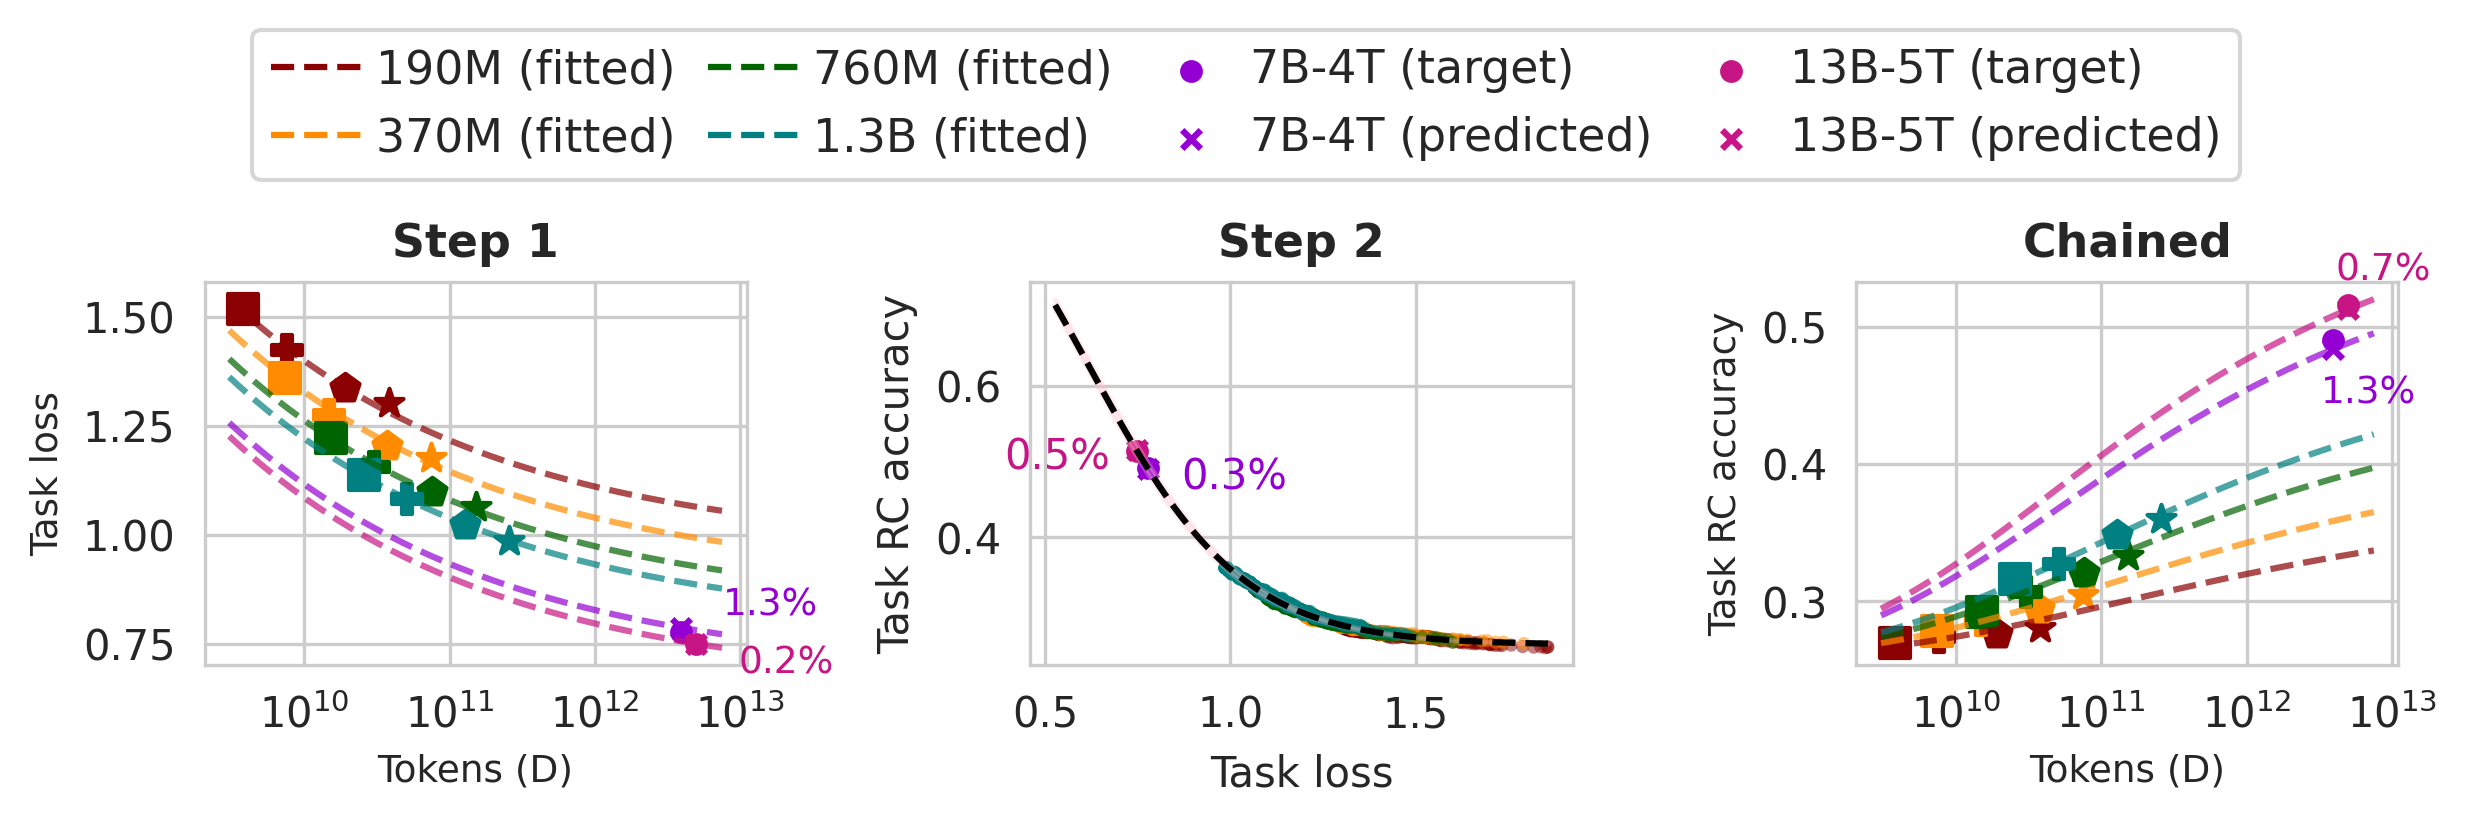
\includegraphics[width=0.9\linewidth]{images/figure1.png}
\vspace{-12pt}
\caption{
    Predicting MMLU accuracy with our method.
    We use model size $N$ and data size $D$ to predict a ``task loss'' on MMLU (step 1), and then use this task loss to predict task accuracy in ranked classification format (step 2).
    The chained plot shows end-to-end prediction from ($N$, $D$) to task accuracy.
    The functions in step 1 and 2 are fitted on data points collected from \textit{ladder} models (markers colored in red, orange, green and cyan); 7B-4T and 13B-5T are the target models for which we make predictions.
    We report relative prediction error in the plot next to each target model point.
    %\pw{fonts in the subplots should be consistent (e.g., step 2 has larger font). These plots would look better if they were taller---I wonder if you could move the legend to the right, and then squeeze the plots horizontally but make them taller?}
}
\label{fig:figure1}
\vspace{-8pt}
\end{figure*}
